\chapter{Insiemi}

\section{Introduzione}

\defn{Insieme}{
La definizione di insieme risale a Cantor (1845-1918): Un \textbf{insieme} è una collezione di oggetti determinati e distinti, detti \textbf{elementi} dell'insieme.
}

Dobbiamo sempre essere in grado di determinare l'appartenenza di un elemento all'insieme.
Gli insiemi si indicano con lettere maiuscole mentre gli elementi di un insieme si indicano con lettere minuscole.

\ex{
\[
C = \{1, 1, 1, 2, 2, 3, 3\} \leftarrow \text{Non è un insieme}
\]
\[
C = \{1, 2, 3\} \leftarrow \text{Gli elementi di un insieme sono distinti}
\]

L'appartenenza e la non appartenenza di un elemento ad un insieme si indicano in questo modo:
\[
a \in A \leftarrow \text{l'elemento } a \text{ appartiene all'insieme } A
\]
\[
a \notin A \leftarrow \text{l'elemento } a \text{ NON appartiene all'insieme } A
\]
}

\subsection{Rappresentazione degli insiemi}
Esistono 3 modi diversi per rappresentare un insieme:
\begin{enumerate}
    \item \textbf{Per elencazione:} $C = \{1, 2, 3\}$
    \item \textbf{Tramite proprietà caratteristica:} $C = \{x \mid x \text{ è un numero primo}\}$
    \item \textbf{Tramite diagramma di Eulero-Venn}
\end{enumerate}


\subsection{Sottoinsiemi}
Dati due insiemi $C$ ed $E$, se tutti gli elementi di $E$ sono contenuti anche in $C$, si dice che $E$ è un sottoinsieme di $C$.
Esistono due tipi di sottoinsiemi:
\begin{itemize}
    \item \textbf{Sottoinsiemi propri:} si indicano con il simbolo $\sub$. Se $E$ è contenuto in $C$ ma $E$ è diverso da $C$, allora $E$ è un sottoinsieme proprio di $C$: $E \sub C$
    \item \textbf{Sottoinsiemi impropri:} si indicano con il simbolo $\sube$. Se $E$ è contenuto in $C$ e $E$ contiene esattamente gli stessi elementi di $C$, allora $E$ è un sottoinsieme improprio di $C$: $E \sube C$
    \item Per indicare che un insieme non è contenuto in un altro insieme si utilizza il simbolo $\notsub$
\end{itemize}

\subsection{Insieme vuoto}
L'\textbf{insieme vuoto} si indica con il simbolo $\emptyset$ ed è, per definizione, contenuto in tutti gli insiemi.

\subsection{Rappresentazione per proprietà caratteristica}

\defn{Proprietà}{
Una \textbf{proprietà} è un'espressione a cui deve essere sempre possibile attribuire un valore di verità (vero o falso). Si indicano con le lettere greche per non confonderle con gli elementi degli insiemi.
}

\subsubsection{Esempi di proprietà}
"Gli $n$ appartenenti ad $\N$ tale che $n$ è un numero pari" $\leftarrow$ Ovvero tale che $n$ renda vera la proprietà $\alpha$ (essere un numero pari):
\[
A = \{n \in \N \mid \alpha\}
\]
Possiamo definire questo insieme senza ricorrere ad $\alpha$ utilizzando la simbologia matematica:
\[
A = \{2n : n \in \N\}
\]


\subsubsection{Riconoscimento di sottoinsiemi tramite proprietà}
Come riconoscere se un insieme è sottoinsieme di un altro se entrambi sono definiti per proprietà?
\begin{itemize}
    \item $\beta$ = essere multiplo di 4
    \item $\alpha$ = essere multiplo di 2
    \item $\gamma$ = essere pari
\end{itemize}

Definiti gli insiemi:
\begin{itemize}
    \item $A = \{n \in \N \mid \beta\}$
    \item $B = \{n \in \N \mid \alpha\}$
    \item $C = \{n \in \N \mid \gamma\}$
\end{itemize}

Possiamo dire che la proprietà $\beta$ implica $\alpha$ e si scrive in questo modo:
\[
\beta \Rightarrow \alpha
\]
(Se è vera $\beta$ è vera anche $\alpha$)
Questo significa che $A \sub B$, poiché ogni multiplo di 4 è anche multiplo di 2.

\section{Quantificatori}

\defn{Quantificatori}{
I \textbf{quantificatori} trasformano gli enunciati aperti in proposizioni che possono assumere il valore di vero o falso.
}

Esistono due tipi di quantificatori:
\begin{itemize}
    \item \textbf{Quantificatore esistenziale:}
    \begin{itemize}
        \item Si indica con il simbolo $\exists$
        \item Indica l'esistenza di almeno un elemento dell'insieme che gode di una particolare proprietà
        \item Il simbolo $\exists!$ indica l'esistenza di uno ed un solo elemento dell'insieme che gode di una particolare proprietà
    \end{itemize}
    \item \textbf{Quantificatore universale:}
    \begin{itemize}
        \item Si indica con il simbolo $\forall$
        \item Indica che tutti gli elementi di un insieme godono della medesima proprietà
    \end{itemize}
\end{itemize}

Riprendiamo le proprietà descritte in precedenza:
\begin{itemize}
    \item $\beta$ = essere multiplo di 4
    \item $\alpha$ = essere multiplo di 2
    \item $\gamma$ = essere pari
\end{itemize}

Definiti gli insiemi:
\[
A = \{n \in \N \mid \alpha\}
\]
\[
B = \{n \in \N \mid \beta\}
\]

Possiamo dire che:
\begin{itemize}
    \item $\exists n \in A : n \in B$ $\leftarrow$ Esiste almeno un numero multiplo di due che è anche multiplo di 4
    \item $\forall n \in B \Rightarrow n \in A$ $\leftarrow$ Ogni multiplo di 4 è anche multiplo di 2
    \item $\nexists n \in B : n \notin A$ $\leftarrow$ Non esiste multiplo di 4 che non sia anche multiplo di 2
\end{itemize}

\section{Operazioni tra insiemi}
Sia $M$ un insieme universo e definiamo gli insiemi $A, B \subseteq M$. Possiamo definire le seguenti operazioni sugli insiemi:

\subsubsection{Unione}
Si indica con $A \cup B = \{x \in M \mid x \in A \lor x \in B\}$.

\subsubsection{Intersezione}
Si indica con $A \cap B = \{x \in M \mid x \in A \land x \in B\}$. Se $A \cap B = \emptyset$ allora $A$ e $B$ sono \textbf{disgiunti} (non hanno elementi in comune).

\subsubsection{Complemento (Differenza)}
Si indica con $A \setminus B = \{x \in A \mid x \notin B\}$.

\subsubsection{Complementare}
Si indica con $\overline{A} = M \setminus A = \{x \in M \mid x \notin A\}$.

\subsection{Proprietà delle operazioni tra insiemi}

\subsubsection{Commutatività di Unione e Intersezione}
\begin{itemize}
    \item $A \cup B = B \cup A$
    \item $A \cap B = B \cap A$
\end{itemize}

\subsubsection{Associatività di Unione e Intersezione}
\begin{itemize}
    \item $(A \cup B) \cup C = A \cup (B \cup C) = A \cup B \cup C$
    \item $(A \cap B) \cap C = A \cap (B \cap C) = A \cap B \cap C$
\end{itemize}

\subsubsection{Distributività}
\begin{itemize}
    \item \textbf{Dell'unione rispetto all'intersezione:}
    \[
    A \cup (B \cap C) = (A \cup B) \cap (A \cup C)
    \]
    \item \textbf{Dell'intersezione rispetto all'unione:}
    \[
    A \cap (B \cup C) = (A \cap B) \cup (A \cap C)
    \]
\end{itemize}

\subsection{Il prodotto cartesiano}
Un insieme è un aggregato caotico di elementi. Non c'è rilevanza sull'ordine degli elementi. Per introdurre l'ordine dobbiamo ricorrere al prodotto cartesiano.

\defn{Coppia Ordinata}{
Siano $A, B \neq \emptyset$, si chiama \textbf{coppia ordinata} di prima componente $a \in A$ e seconda componente $b \in B$ il seguente oggetto: $(a, b) \neq (b, a)$.
}

\defn{Prodotto Cartesiano}{
Si definisce \textbf{prodotto cartesiano} di $A \times B$ l'insieme di tutte le possibili coppie $A \times B = \{(a, b) \mid a \in A, b \in B\}$.
}

\ex{
Poniamo $A = \{a, b\}$ e $B = \{c, d\}$:

$A \times B = \{(a, c), (a, d), (b, c), (b, d)\}$ $\leftarrow$ Tutte le coppie con prima componente in $A$

$B \times A = \{(c, a), (c, b), (d, a), (d, b)\}$ $\leftarrow$ Tutte le coppie con prima componente in $B$

Ne consegue che il prodotto cartesiano non è commutativo, difatti $A \times B \neq B \times A$.
Il prodotto cartesiano $A \times A$ si indica con $A^2$.
}

\section{Relazioni e ordinamenti}

\subsection{Relazione}

\defn{Relazione}{
Siano $A, B \ne \emptyset$. Si chiama \textbf{relazione} e si indica con $\mathcal{R}$ una proprietà definita sul prodotto cartesiano $A \times B$.
Per una coppia di elementi $(a, b)$ posso stabilire se $\mathcal{R}$ assume valore vero o falso.
Ci sarà quindi un sottoinsieme di $A \times B$ contenente le coppie che soddisfano la relazione.
}

Per dire che una coppia $(a, b)$ verifica la relazione $\mathcal{R}$, scriveremo $a \mathcal{R} b$ (a è in relazione con b).
La relazione $\mathcal{R}$ su $A^2$ si dice \textbf{binaria}. Una relazione binaria è quindi definita su un unico insieme A. Formalmente: $\mathcal{R} \subseteq A \times A$.

Sulle relazioni binarie è possibile definire alcune proprietà.


\subsubsection{Proprietà delle Relazioni Binarie}
Sia $A \ne \emptyset$ e $\mathcal{R}$ una relazione binaria su $A^2$ (cioè $A \times A$). Allora valgono le seguenti definizioni:

\begin{itemize}
    \item $\mathcal{R}$ si dice \textbf{riflessiva} se e solo se $\forall x \in A$, $x \mathcal{R} x$.
    \textbf{Esempio:}
    \begin{tcolorbox}[colback=gray!10, arc=0mm, boxrule=0.5pt, left=2mm, right=2mm, top=1mm, bottom=1mm]
      Sull'insieme $A = \{1, 2, 3\}$, la relazione "$\leq$" è riflessiva perché $1 \leq 1$, $2 \leq 2$, $3 \leq 3$.
    \end{tcolorbox}

    \item $\mathcal{R}$ si dice \textbf{simmetrica} se e solo se $\forall x, y \in A$, $x \mathcal{R} y \implies y \mathcal{R} x$.
    \textbf{Esempio:}
    \begin{tcolorbox}[colback=gray!10, arc=0mm, boxrule=0.5pt, left=2mm, right=2mm, top=1mm, bottom=1mm]
      Sull'insieme $\mathbb{Z}$ dei numeri interi, la relazione "è congruo modulo 2 a" (ovvero "$x \equiv y \pmod{2}$") è simmetrica: se $3 \equiv 5 \pmod{2}$, allora $5 \equiv 3 \pmod{2}$.
    \end{tcolorbox}

    \item $\mathcal{R}$ si dice \textbf{transitiva} se e solo se $\forall x, y, z \in A$, $x \mathcal{R} y$ e $y \mathcal{R} z \implies x \mathcal{R} z$.
    \textbf{Esempio:}
    \begin{tcolorbox}[colback=gray!10, arc=0mm, boxrule=0.5pt, left=2mm, right=2mm, top=1mm, bottom=1mm]
      Sull'insieme dei numeri, la relazione "$\leq$" è transitiva: se $1 \leq 2$ e $2 \leq 3$, allora $1 \leq 3$.
    \end{tcolorbox}

    \item $\mathcal{R}$ si dice \textbf{antisimmetrica} se e solo se $\forall x, y \in A$, $x \mathcal{R} y$ e $y \mathcal{R} x \implies x = y$.
    \textbf{Esempio:}
    \begin{tcolorbox}[colback=gray!10, arc=0mm, boxrule=0.5pt, left=2mm, right=2mm, top=1mm, bottom=1mm]
      La relazione "$\leq$" sui numeri naturali è antisimmetrica: se $x \leq y$ e $y \leq x$, allora necessariamente $x = y$.
    \end{tcolorbox}
\end{itemize}

\defn{Relazione d'Ordine}{
Una relazione $\mathcal{R}$ su $A^2$ si dice \textbf{relazione d'ordine} se è:
\begin{itemize}
    \item Riflessiva
    \item Transitiva
    \item Antisimmetrica
\end{itemize}
In questo caso si indica con il simbolo $\leq$.
}

\defn{Relazione di Equivalenza}{
Una relazione $\mathcal{R}$ su $A^2$ si dice \textbf{relazione di equivalenza} se è:
\begin{itemize}
    \item Riflessiva
    \item Transitiva
    \item Simmetrica
\end{itemize}
Si indica con il simbolo $\sim$.
}

\subsection{Massimo e minimo}

\rmk{
Sia $M$ un insieme non vuoto ($M \ne \emptyset$) su cui sia definita la relazione $\leq$. Sia $A \subseteq M$, $A \ne \emptyset$. $\underline{m} \in A$ si dice \textbf{MINIMO} di $A$ se $\underline{m} \leq a \forall a \in A$. Analogamente, $\overline{m} \in A$ si dice \textbf{MASSIMO} di $A$ se $a \leq \overline{m}, \forall a \in A$.
}

\rmk{
Non è detto che esistano ($\exists$), ma se esistono, sono unici. Si denotano come segue:
\[
\min A \in A \quad\text{e}\quad \max A \in A
\]
}

\pf{
Procediamo per assurdo, supponendo che il minimo $\underline{m}$ (che esiste per ipotesi) \textbf{non sia unico}:
\begin{enumerate}
    \item Sia $\underline{a} \in A$ un altro candidato minimo
    \item Per definizione di minimo: $\underline{a} \leq a$, $\forall a \in A$
    \item In particolare: $\underline{a} \leq \underline{m}$
    \item Ma essendo $\underline{m}$ minimo: $\underline{m} \leq \underline{a}$
    \item Essendo la relazione $\leq$ \textbf{antisimmetrica}, segue che $\underline{a} = \underline{m}$ → Dimostrata l’unicità del minimo
\end{enumerate}

\textbf{Dimostrazione dell'unicità del massimo}

Procediamo per assurdo, supponendo che il massimo $\overline{m}$ (che esiste per ipotesi) \textbf{non sia unico}:
\begin{enumerate}
    \item Sia $\overline{a} \in A$ un altro candidato massimo
    \item Per definizione di massimo: $a \leq \overline{a}$, $\forall a \in A$
    \item In particolare: $\overline{m} \leq \overline{a}$
    \item Ma essendo $\overline{m}$ massimo: $\overline{a} \leq \overline{m}$
    \item Essendo la relazione $\leq$ \textbf{antisimmetrica}, segue che $\overline{a} = \overline{m}$ → Dimostrata l’unicità del massimo
\end{enumerate}
}

\subsection{Maggiorante e Minorante}
Sia $M$ un insieme ordinato dove è definita la relazione d'ordine $\leq$, sia $A \subseteq M$, $A \ne \emptyset$:
$\underline{x} \in M$ si dice \textbf{minorante} di $a$ se $\underline{x} \leq a \forall a \in A$, esempio:
\begin{itemize}
    \item Nell'intervallo $]-1, 2]$ il minorante è $-1$, mentre $2$ è il massimo
\end{itemize}
Analogamente, $\overline{x} \in M$ si dice \textbf{maggiorante} di $a$ se $a \leq \overline{x} \forall a \in A$

\rmk{
\textbf{Osservazione:} Maggiorante e minorante, se esistono, non è detto che siano unici.
}

\defn{Insieme Limitato}{
$A \subseteq M$ si dice:
\begin{itemize}
    \item \textbf{Inferiormente limitato} se ammette minoranti.
    \item \textbf{Superiormente limitato} se ammette maggioranti.
    \item \textbf{Limitato} se è sia inferiormente che superiormente limitato.
\end{itemize}
}

\subsection{Estremo Superiore ed Estremo Inferiore}

\defn{Estremo Inferiore e Superiore}{
Sia $A \subseteq M$, $A \ne \emptyset$, con $A$ \textbf{inferiormente limitato} (cioè esiste almeno un minorante).
Se l'insieme dei minoranti ammette massimo, esso si chiama $\inf A$ (\textbf{estremo inferiore} di $A$).
Analogamente, se $A$ è \textbf{superiormente limitato} e l'insieme dei maggioranti ammette minimo, esso si chiama $\sup A$ (\textbf{estremo superiore} di $A$).
}

Se esistono $\min A$ e $\max A$, allora si ha:
\[
\min A = \inf A \quad \text{e} \quad \max A = \sup A
\]
Questo implica:
\begin{itemize}
    \item Se $\max A$ esiste, allora $\sup A = \max A$ e $A$ è superiormente limitato.
    \item Se $\min A$ esiste, allora $\inf A = \min A$ e $A$ è inferiormente limitato.
\end{itemize}

\subsection{Insiemi completi}

\defn{Insieme Completo}{
Sia $M$ un insieme ordinato.
$M$ si dice \textbf{completo} se ogni suo sottoinsieme non vuoto e superiormente limitato ammette $\sup$.
In maniera equivalente, $M$ è completo se ogni sottoinsieme non vuoto e inferiormente limitato ammette $\inf$.
}

\section{Insiemi numerici}

Per introdurre gli insiemi numerici si possono seguire due approcci:
\begin{itemize}
\item partire da $\mathbb{N}$ e costruire progressivamente $\mathbb{Z}, \mathbb{Q}, \mathbb{R}$;
\item partire da $\mathbb{R}$ come corpo ordinato completo e definire a posteriori $\mathbb{N}, \mathbb{Z}, \mathbb{Q}$ come suoi sottoinsiemi.
\end{itemize}


\subsubsection{Partendo da $\mathbb{N}$}
Si postula l'esistenza dell'insieme $\mathbb{N}$ dei numeri naturali, su cui sono definite due operazioni fondamentali: l'addizione e la moltiplicazione.

\defn{Operazione}{
Si chiama \emph{operazione} una funzione
\[
\sigma : \mathbb{N} \times \mathbb{N} \to \mathbb{N}, \qquad (n,m) \mapsto n \,\sigma\, m .
\]
}

Le operazioni di base che assumiamo in $\mathbb{N}$ sono
\[
(\mathbb{N}, +, \cdot).
\]

La sottrazione e la divisione non sono sempre definite in $\mathbb{N}$; per introdurle occorre ampliare l’insieme.

- Estendendo $\mathbb{N}$ si ottiene l’insieme degli interi:
  \[
  \mathbb{Z} = \mathbb{N}_{0} \cup (-\mathbb{N}),
  \]
  in cui sono ben definite le operazioni $+$ e $-$.
- Per permettere la divisione si introduce l’insieme dei razionali:
  \[
  \mathbb{Q} = \left\{ \tfrac{m}{n} \;\middle|\; m \in \mathbb{Z}, \; n \in \mathbb{Z}\setminus\{0\} \right\}.
  \]

Tuttavia $\mathbb{Q}$ non è ancora sufficiente: ad esempio $\sqrt{2} \notin \mathbb{Q}$.

\prop{
Non esiste alcun $c \in \mathbb{Q}$ tale che $c^2 = 2$.

}

\pf{
Supponiamo per assurdo che $c = \tfrac{p}{q}$ con $p,q \in \mathbb{N}$ primi tra loro e $c^2 = 2$.
Allora $p^2 = 2q^2$, quindi $p^2$ è pari $\implies$ $p$ è pari. Scriviamo $p = 2k$:
\[
p^2 = 4k^2 = 2q^2 \implies q^2 = 2k^2,
\]
quindi anche $q$ è pari. Ma se $p$ e $q$ sono entrambi pari, non possono essere primi tra loro. Contraddizione.
}

Segue che $\sqrt{2} \notin \mathbb{Q}$, e quindi è necessario introdurre l’insieme dei numeri reali $\mathbb{R}$.


\subsubsection{Costruzione dei numeri reali}
Si postula l’esistenza di un insieme $\mathbb{R}$ che soddisfa una lista di assiomi.
Gli assiomi si dividono in tre categorie:
\begin{enumerate}[label=\Alph*)]
\item assiomi relativi alle operazioni ($+, \cdot$);
\item assiomi relativi all’ordinamento;
\item assioma di completezza.
\end{enumerate}

Un insieme con queste proprietà è detto \emph{corpo ordinato completo} e, a meno di isomorfismo, è unico: lo identifichiamo con $\mathbb{R}$.

\subsubsection{Assiomi relativi alle operazioni}
In $\mathbb{R}$ sono definite due operazioni:
\begin{itemize}
\item Somma \quad $+ : (a, b) \in \mathbb{R}^2 \mapsto a + b \in \mathbb{R}$
\item Prodotto \quad $\cdot : (a, b) \in \mathbb{R}^2 \mapsto a \cdot b \in \mathbb{R}$
\end{itemize}

Queste operazioni verificano le seguenti proprietà:
\begin{enumerate}
  \renewcommand{\labelenumi}{a\theenumi}

  \item Proprietà commutativa
  \[
    a + b = b + a \quad \forall a, b \in \mathbb{R}
  \]
  \[
    a \cdot b = b \cdot a \quad \forall a, b \in \mathbb{R}
  \]

  \item Proprietà associativa
  \[
    a + (b + c) = (a + b) + c \quad \forall a, b, c \in \mathbb{R}
  \]
  \[
    a \cdot (b \cdot c) = (a \cdot b) \cdot c \quad \forall a, b, c \in \mathbb{R}
  \]

  \item Proprietà distributiva
  \[
    a \cdot (b + c) = a \cdot b + a \cdot c \quad \forall a, b, c \in \mathbb{R}
  \]

  \item Esistenza degli elementi neutri
  \[
    \exists\, 0 \in \mathbb{R} \;\; \text{tale che} \;\; a + 0 = a \quad \forall a \in \mathbb{R}
  \]
  \[
    \exists\, 1 \in \mathbb{R} \;\; \text{tale che} \;\; a \cdot 1 = a \quad \forall a \in \mathbb{R}
  \]

  \item Esistenza degli opposti e degli inversi
  \[
    \forall a \in \mathbb{R}, \; \exists (-a) \in \mathbb{R} \;\; \text{tale che} a+(-a) = 0
  \]
  \[
    \forall a \in \mathbb{R}\setminus \{0\}, \; \exists a^{-1} \in \mathbb{R} \;\; \text{tale che} \;\; a \cdot a^{-1} = 1
  \]
\end{enumerate}

Al momento, la struttura $(\mathbb{R}, +, \cdot)$ forma un campo.

\paragraph{Osservazione.}
Alcune conseguenze degli assiomi relativi alle operazioni:
possiamo definire due nuove operazioni come derivate da $+$ e $\cdot$:

\begin{itemize}
\item Sottrazione \quad $a - b := a + (-b) \quad \forall a, b \in \mathbb{R}$
\item Divisione \quad $a : b := a \cdot b^{-1} \quad \forall a \in \mathbb{R}, \; b \in \mathbb{R}\setminus \{0\}$
\end{itemize}

\prop{
Per ogni $a \in \mathbb{R}$ vale
\[
a \cdot 0 = 0.
\]
}

\pf{
Sia $x \in \mathbb{R}$.
Per la proprietà dell’elemento neutro additivo (a4) abbiamo
\[
x \cdot 0 = x \cdot (0 + 0).
\]
Per la distributività (a3):
\[
x \cdot (0 + 0) = x \cdot 0 + x \cdot 0.
\]
Sottraiamo $x \cdot 0$ da entrambi i membri (per l’esistenza dell’opposto, a5):
\[
x \cdot 0 = x \cdot 0 + x \cdot 0 \;\;\implies\;\; 0 = x \cdot 0.
\]
Quindi $a \cdot 0 = 0$ per ogni $a \in \mathbb{R}$.
}

\subsubsection{Assiomi relativi all'ordinamento}
Si assume che in $\mathbb{R}$ esista una relazione d’ordine $\leq$, cioè una relazione d’ordine riflessiva, antisimmetrica, transitiva e totale.
In altre parole, per ogni $a,b \in \mathbb{R}$ vale $a \leq b$ oppure $b \leq a$.

Questa relazione è definita su $\mathbb{R}$ e verifica i seguenti assiomi:

\begin{enumerate}
  \renewcommand{\labelenumi}{b\theenumi}

  \item Compatibilità rispetto alla somma:
  \[
    \forall a,b,c \in \mathbb{R}, \; a \leq b \;\;\implies\;\; a+c \leq b+c.
  \]

  \item Compatibilità rispetto al prodotto:
  \[
    \forall a,b \in \mathbb{R}, \; \forall c \in \mathbb{R}, \;
    a \leq b \;\wedge\; 0 \leq c \;\;\implies\;\; a \cdot c \leq b \cdot c.
  \]
\end{enumerate}

L'oggetto $(\mathbb{R}, +, \cdot, \leq)$ prende il nome di \emph{campo ordinato}.
\subsubsection{Altre importanti conseguenze}
Le altre due conseguenze fondamentali legate al fatto che abbiamo una relazione d'ordine totale sono le seguenti proprietà:
\prop{Caratterizzazione di $\sup$ e $\inf$}{
\begin{enumerate}
  \item
      Sia $A \subseteq \mathbb{R}$ con $A \neq \emptyset$.
      Allora $C \in \mathbb{R}$ è il supremo di $A$ ($C = \sup A$) se e solo se valgono le seguenti proprietà:
      \begin{enumerate}
        \item $\forall a \in A, \; a \leq C$
        \item $\forall \epsilon > 0, \; \exists a_\epsilon \in A \;|\; C - \epsilon < a_\epsilon$
      \end{enumerate}
  \item
      Sia $A \subseteq \mathbb{R}$ con $A \neq \emptyset$.
      Allora $c \in \mathbb{R}$ è l'infimo di $A$ ($c = \inf A$) se e solo se valgono le seguenti proprietà:
      \begin{enumerate}
        \item $\forall a \in A, \; c \leq a$
        \item $\forall \epsilon > 0, \; \exists a_\epsilon \in A \;|\; a_\epsilon < c + \epsilon$
      \end{enumerate}
  \end{enumerate}
}

\pf{
Dobbiamo dimostrare la doppia implicazione. Per definizione di $\sup$ (\nameref{estremi}) la 1 è ovvia
(dato che $\sup$ è il minimo dei maggioranti).

Dimostrazione $\implies$:

Per dimostrare la 2, prendiamo $\epsilon > 0$ arbitrario e consideriamo $C - \epsilon \in \R$.
È chiaro che $C - \epsilon < C$, dato che la relazione d’ordine è totale.

Poiché $C$ è il minimo dei maggioranti, $C - \epsilon$ non può essere un maggiorante di $A$.
Dunque $\exists a_{\epsilon} \in A$ tale che $C - \epsilon < a_{\epsilon} \leq C$.
Attenzione però: questo non significa che $a_{\epsilon}$ sia un maggiorante, ma solo che “si avvicina” a $C$ dal basso.

Dimostrazione $\impliedby$:

Dimostriamo che se $C \in \R$ verifica la 1 e la 2, allora $C$ è il $\sup$ di $A$, cioè:

\begin{enumerate}
\item $C$ è un maggiorante di $A$,
\item $C$ è il minimo dei maggioranti.
\end{enumerate}

Come prima, la 1 è ovvia. Dimostriamo la 2 per assurdo.

Supponiamo che esista $C' < C$ che sia un maggiorante di $A$.
Allora $C' = C - \epsilon$ con $\epsilon > 0$.
Ma per la condizione 2 sappiamo che $\exists a_{\epsilon} \in A$ tale che $C - \epsilon < a_{\epsilon}$, cioè $C' < a_{\epsilon}$.
Questo contraddice il fatto che $C'$ sia un maggiorante di $A$.

Quindi $C$ è il minimo dei maggioranti, cioè $C = \sup A$.
}

\pf{
Dobbiamo dimostrare l’analogo per l’$\inf$. Per definizione di $\inf$ la 1 è ovvia
(dato che $\inf$ è il massimo dei minoranti).

Dimostrazione $\implies$:

Sia $C = \inf A$. Per mostrare la 2 prendiamo $\epsilon > 0$ arbitrario e consideriamo $C + \epsilon \in \R$.
È chiaro che $C < C + \epsilon$.

Poiché $C$ è il massimo dei minoranti, $C + \epsilon$ non può essere un minorante di $A$.
Dunque $\exists a_{\epsilon} \in A$ tale che $C \leq a_{\epsilon} < C + \epsilon$.
Attenzione: questo non significa che $a_{\epsilon}$ sia un minorante, ma solo che “si avvicina” a $C$ dall’alto.

Dimostrazione $\impliedby$:

Dimostriamo che se $C \in \R$ verifica la 1 e la 2, allora $C$ è l’$\inf$ di $A$, cioè:

\begin{enumerate}
\item $C$ è un minorante di $A$,
\item $C$ è il massimo dei minoranti.
\end{enumerate}

La 1 è ovvia. Dimostriamo la 2 per assurdo.
Supponiamo che esista $C' > C$ che sia un minorante di $A$.
Allora $C' = C + \epsilon$ con $\epsilon > 0$.
Ma per la condizione 2 sappiamo che $\exists a_{\epsilon} \in A$ tale che $a_{\epsilon} < C + \epsilon = C'$, con $a_{\epsilon} \geq C$.
Quindi $a_{\epsilon} \not\geq C'$, contraddicendo il fatto che $C'$ fosse un minorante.

Quindi $C$ è il massimo dei minoranti, cioè $C = \inf A$.
}

\subsubsection{Assioma di completezza}
Per $\mathbb{R}$ vale il seguente assioma:
\fact{
$\mathbb{R}$ è un insieme completo: ogni $A \subseteq \mathbb{R}$ superiormente limitato ammette estremo superiore $\iff$ ogni $A \subseteq \mathbb{R}$ inferiormente limitato ammette estremo inferiore (\nameref{estremi}).
}

Denotiamo con $(\mathbb{R}, +, \cdot, \leq, \text{Assioma di completezza})$ il campo dei numeri reali.

Costruiamo i sottoinsiemi numerici:
\begin{itemize}
  \item $\mathbb{N}$: insieme dei numeri naturali, il più piccolo sottoinsieme di $\mathbb{R}$ che contiene l’unità e il successivo di ogni suo elemento:
    \[
    \forall n \in \mathbb{N},\quad n+1 \in \mathbb{N}.
    \]
  \item $\mathbb{N}_0 = \mathbb{N} \cup \{0\}$.
  \item $\mathbb{Z} = \mathbb{N}_0 \cup (-\mathbb{N})$.
  \item $\mathbb{Q} = \left\{\tfrac{n}{m} \;\middle|\; n \in \mathbb{Z},\ m \in \mathbb{Z}\setminus\{0\}\right\}$.
\end{itemize}

Si ha la catena di inclusioni:
\[
\mathbb{N} \subset \mathbb{N}_0 \subset \mathbb{Z} \subset \mathbb{Q} \subseteq \mathbb{R}.
\]

\prop{
L’insieme $\mathbb{Q}$ non è completo; ne consegue che $\mathbb{Q} \subset \mathbb{R}$ (inclusione propria), ovvero $\mathbb{R}\setminus\mathbb{Q} \neq \emptyset$.
}

\pf{
  \rmk{
    Questa è una dimostrazione costruttiva, ovvero ci darà altre informazioni oltre a verificare la tesi.
  }
  Per dimostrare che $\mathbb{Q}$ non soddisfa l’assioma di completezza, basta costruire un controesempio:

  Voglio costruire un insieme superiormente limitato dove il sup è uguale a $\sqrt{2}$

Consideriamo l’insieme
\[
A = \{ r \in \mathbb{Q} \mid r > 0,\ r^2 \leq 2 \}.
\]

$A$ è limitato superiormente, sia visto come sottoinsieme di $\mathbb{Q}$ che di $\mathbb{R}$.

In $\mathbb{R}$, per l’assioma di completezza, esiste $c = \sup A$. È facile vedere che $c = \sqrt{2}$.
Poiché $\sqrt{2} \notin \mathbb{Q}$, concludiamo già che $\sup A \notin \mathbb{Q}$.

Ora analizziamo i maggioranti di $A$ in $\mathbb{Q}$:
\[
B = \{ p \in \mathbb{Q} \mid p > 0,\ p^2 > 2 \}.
\]

$B$ è l’insieme dei maggioranti razionali di $A$. Dimostriamo che $B$ non ha minimo.

Dato un qualsiasi $p \in B$, costruiamo
\[
q = p - \frac{p^2-2}{p+2}.
\]
Ovvero un elemento più piccolo di $p$.

Allora:
\begin{itemize}
  \item $q < p$;
  \item $q \in \mathbb{Q}$ (perché è ottenuto da operazioni razionali su $p$);
  \item $q^2 - 2 = \frac{2(p^2-2)}{(p+2)^2} > 0 \quad\implies\quad q^2 > 2$.
\end{itemize}

Quindi $q \in B$ ed è più piccolo di $p$. Dunque $B$ non ammette minimo.

Conclusione: l’insieme $A \subseteq \mathbb{Q}$ è superiormente limitato ma non ha $\sup$ in $\mathbb{Q}$.
Quindi $\mathbb{Q}$ non è completo, mentre in $\mathbb{R}$ lo stesso insieme ha estremo superiore $\sqrt{2} \in \mathbb{R} \setminus \mathbb{Q}$.
}

\subsection{Proprietà dei numeri Naturali}

\prop{
$\N$ non è superiormente limitato.
}

\pf{
Supponiamo per assurdo che $\N$ sia superiormente limitato.
Allora, essendo $\N \subseteq \R$, per l’assioma di completezza esiste $c = \sup \N$.

Per le proprietà del $\sup$, preso $\varepsilon = 1$, esiste $S \in \N$ tale che
\[
c - 1 < S \leq c.
\]
Ma allora $S+1 \in \N$ e vale $S+1 > c$, in contraddizione con il fatto che $c$ sia un maggiorante.

Dunque $\N$ non è superiormente limitato.
}

\cor{
Poiché $\N \subseteq \Z \subseteq \Q \subseteq \R$, anche $\Z$, $\Q$ e $\R$ non sono superiormente limitati.
}

\rmk{
Se $A \subseteq \R$ non è superiormente limitato, poniamo $\sup A = +\infty$.
Analogamente, se $A$ non è inferiormente limitato, poniamo $\inf A = -\infty$.

L’insieme $\R \cup \{+\infty,-\infty\}$ si chiama \textbf{reale esteso}.
}

\prop{
Sia $A \subseteq \R$, $A \neq \emptyset$.
Allora
\[
\sup A = +\infty \iff \forall k > 0, \; \exists a_k \in A \; \text{tale che } a_k > k.
\]
}

\prop{
Sia $A \subseteq \R$, $A \neq \emptyset$.
Allora
\[
\inf A = -\infty \iff \forall k > 0, \; \exists a_k \in A \; \text{tale che } a_k < -k.
\]
}

\subsection{Insiemi separati e contigui}
Per completare il discorso su $\inf$ e $\sup$, introduciamo due definizioni fondamentali.
\defn{Insiemi separati}{
 Siano $A,B \subseteq \mathbb{R}$, $A,B \neq \emptyset$.
  Diremo che $A$ e $B$ sono \textbf{separati} se
  \[
  \forall a \in A, \, \forall b \in B \implies a \leq b.
  \]
}

\defn{Insiemi contigui}{
 Diremo che $A$ e $B$ sono \textbf{contigui} se sono separati e, in più, per ogni $\varepsilon > 0$ esistono $a_\varepsilon \in A$, $b_\varepsilon \in B$ tali che
  \[
  b_\varepsilon - a_\varepsilon < \varepsilon.
  \]
}

Esempio con i seguenti intervalli:
\begin{itemize}
\item $]1, 2[$
\item $]2, 3[$
\item $]3, 4[$
\end{itemize}

Gli intervalli $]1, 2[$ e $]3, 4[$ sono separati, mentre $]2,3[$ è contiguo sia a $]1,2[$ che a $]3,4[$.

\begin{center}
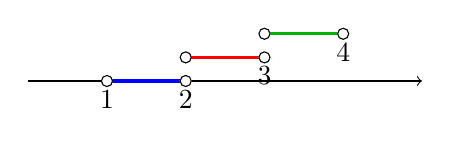
\begin{tikzpicture}
  % asse dei numeri
  \draw[->] (0,0) -- (5,0);

  % intervallo (1,2)
  \draw[very thick, blue] (1,0) -- (2,0);
  \filldraw[white] (1,0) circle (2pt);
  \draw (1,0) circle (2pt);
  \filldraw[white] (2,0) circle (2pt);
  \draw (2,0) circle (2pt);

  % intervallo (2,3)
  \draw[very thick, red] (2,0.3) -- (3,0.3);
  \filldraw[white] (2,0.3) circle (2pt);
  \draw (2,0.3) circle (2pt);
  \filldraw[white] (3,0.3) circle (2pt);
  \draw (3,0.3) circle (2pt);

  % intervallo (3,4)
  \draw[very thick, green!70!black] (3,0.6) -- (4,0.6);
  \filldraw[white] (3,0.6) circle (2pt);
  \draw (3,0.6) circle (2pt);
  \filldraw[white] (4,0.6) circle (2pt);
  \draw (4,0.6) circle (2pt);

  % etichette
  \node[below] at (1,0) {$1$};
  \node[below] at (2,0) {$2$};
  \node[below] at (3,0.3) {$3$};
  \node[below] at (4,0.6) {$4$};
\end{tikzpicture}
\end{center}

Possiamo quindi dire che due insiemi sono contigui quando il $\sup$ del primo coincide con l’$\inf$ del secondo.

\thm{Elemento di separazione}{
Siano $A,B \subseteq \mathbb{R}$, $A,B \neq \emptyset$.
  Allora $A$ e $B$ sono contigui $\iff \sup A = \inf B = c$.
  Tale $c$ si dice \textbf{elemento di separazione}.
}

\pf{
$\implies$:


  Se $A$ e $B$ sono contigui, allora sono anche separati.
  Quindi $A$ è superiormente limitato da ogni $b \in B$ e $B$ è inferiormente limitato da ogni $a \in A$.
  Per completezza di $\mathbb{R}$ esistono $\sup A = c$ e $\inf B = c'$.
  Per definizione di contiguità: per ogni $\varepsilon>0$ esistono $a_\varepsilon \in A$, $b_\varepsilon \in B$ con $b_\varepsilon - a_\varepsilon < \varepsilon$.
  Ma allora $0 \leq c'-c \leq b_\varepsilon - a_\varepsilon < \varepsilon$.
  Poiché $\varepsilon$ è arbitrario, segue $c=c'$.

  $\impliedby$:


  Viceversa, se $\sup A = \inf B = c$, allora per ogni $\varepsilon > 0$:
  \[
  \exists a_\varepsilon \in A : c - \tfrac{\varepsilon}{2} < a_\varepsilon \leq c, \quad
  \exists b_\varepsilon \in B : c \leq b_\varepsilon < c + \tfrac{\varepsilon}{2}.
  \]
  Dunque
  \[
  0 \leq b_\varepsilon - a_\varepsilon < \varepsilon.
  \]
  Quindi $A$ e $B$ sono contigui.
}

\subsection{Cardinalità}

\defn{Equipotenza}{
Due insiemi $A$ e $B$ si dicono \textbf{equipotenti} se esiste una biiezione $f : A \to B$ (cioè $f$ è iniettiva e suriettiva).
}

\defn{Insieme finito}{
Un insieme $A \subseteq \mathbb{R}$ si dice \textbf{finito} se esiste $n \in \mathbb{N}$ tale che $A$ è equipotente all’insieme $\{1,2,\dots,n\}$.
  In tal caso $n$ si dice \textbf{cardinalità} di $A$.
}

\defn{Insieme infinito e numerabile}{
Un insieme $A$ si dice \textbf{infinito} se è equipotente ad una sua parte propria.
  Ad esempio, $\mathbb{N}$ è infinito: infatti è equipotente all’insieme $2\mathbb{N} = \{2n : n \in \mathbb{N}\}$ tramite la funzione $f(n) = 2n$.

  La cardinalità di $\mathbb{N}$ si chiama \textbf{numerabile}.
}

\rmk{
 L’insieme $\mathbb{R}$ non è numerabile. Più precisamente, l’intervallo $[0,1] \subseteq \mathbb{R}$ non è numerabile (dimostrazione di Cantor).
  La cardinalità di $\mathbb{R}$ si dice \textbf{potenza del continuo}.
}

\prop{
Per ogni $x > 0$ e $y \in \mathbb{R}$ esiste $n \in \mathbb{N}$ tale che $nx > y$.
  Equivalentemente, per ogni $y > 0$ esiste $n \in \mathbb{N}$ con $1/n < y$.
}

\defn{Densità di $\mathbb{Q}$ in $\mathbb{R}$}{
Dati $a,b \in \mathbb{R}$ con $a < b$, esiste $r \in \mathbb{Q}$ tale che $a < r < b$.
}

\rmk{
 L’insieme $\mathbb{N}$ non ha la proprietà di densità: ad esempio tra $1$ e $2$ non ci sono infiniti naturali, mentre tra due reali ci sono sempre infiniti razionali.
}

\pf{
}

\subsection{Rappresentazione geometrica di $\mathbb{R}$}
In $\mathbb{R}$ ci sono sottoinsiemi particolarmente importanti chiamati \textbf{intervalli}. Essi rappresentano insiemi di numeri compresi tra due estremi, eventualmente inclusi o esclusi.

\paragraph{Intervalli limitati}

\begin{itemize}
  \item $]a,b[ = \{ x \in \mathbb{R} \mid a < x < b \}$ (aperto)
  \item $[a,b] = \{ x \in \mathbb{R} \mid a \le x \le b \}$ (chiuso)
  \item $]a,b] = \{ x \in \mathbb{R} \mid a < x \le b \}$ (semiaperto a sinistra)
  \item $[a,b[ = \{ x \in \mathbb{R} \mid a \le x < b \}$ (semiaperto a destra)
\end{itemize}

\paragraph{Intervalli illimitati}

\begin{itemize}
  \item $]a, +\infty[ = \{ x \in \mathbb{R} \mid x > a \}$ (aperto a sinistra, illimitato a destra)
  \item $[a, +\infty[ = \{ x \in \mathbb{R} \mid x \ge a \}$ (chiuso a sinistra, illimitato a destra)
  \item $]-\infty, b[ = \{ x \in \mathbb{R} \mid x < b \}$ (illimitato a sinistra, aperto a destra)
  \item $]-\infty, b] = \{ x \in \mathbb{R} \mid x \le b \}$ (illimitato a sinistra, chiuso a destra)
  \item $]-\infty, +\infty[ = \mathbb{R}$ (illimitato su entrambi i lati)
\end{itemize}

\section{Principio di induzione}
Se volessi dimostrare:
\begin{itemize}
\item formule su $n!$,
\item proprietà su $x^n$,
\item monotonia: $0 < x_1 < x_2 \implies x_1^n < x_2^n$,
\end{itemize}

è complicato dimostrare una proposizione per infiniti casi.
Abbiamo bisogno del principio di induzione per dimostrare affermazioni che dipendono dagli indici naturali.

Ci sono due variazioni, vedremo la versione classica.

Sia $I \subseteq \mathbb{N}$ che verifica le seguenti proprietà:
\begin{enumerate}
\item $1 \in I$ (base di induzione);
\item se $n \in I \implies n+1 \in I$, allora $I = \mathbb{N}$ (principio di induzione).
\end{enumerate}

\prop{Progressione aritmetica}{
Per ogni $n \in \mathbb{N}$ si ha
\[
1 + 2 + 3 + \dots + n = \frac{n(n+1)}{2},
\]
cioè
\[
\sum_{k=1}^{n} k = \frac{n(n+1)}{2}.
\]
}

\prop{Potenza n-esima}{
Per ogni $n \in \mathbb{N}$ e $x \in \mathbb{R}$ si definisce $x^n$ come:
\begin{itemize}
\item $x^1 = x$,
\item $x^n = x \cdot x^{\,n-1}$ per $n > 1$.
\end{itemize}
}

\prop{Progressione geometrica}{
Per ogni $x \in \mathbb{R}$, $x \neq 1$, si ha
\[
1 + x + x^2 + \dots + x^n = \frac{1 - x^{\,n+1}}{1 - x},
\]
cioè
\[
\sum_{k=0}^{n} x^k = \frac{1 - x^{\,n+1}}{1 - x}.
\]
}

\pf{
Vogliamo dimostrare che per ogni $n \in \mathbb{N}$ e $x \in \mathbb{R}$ con $x \neq 1$ si ha
\[
1 + x + x^2 + \dots + x^n = \frac{1 - x^{\,n+1}}{1-x}.
\]

\textbf{Base di induzione:} per $n=0$ vale
\[
1 = \frac{1 - x^{\,0+1}}{1-x} = \frac{1-x}{1-x} = 1.
\]
Quindi la formula è verificata per $n=0$.

\textbf{Passo induttivo:} supponiamo che la formula sia vera per un certo $n \geq 0$, cioè
\[
1 + x + x^2 + \dots + x^n = \frac{1 - x^{\,n+1}}{1-x}.
\]
Dimostriamo che vale anche per $n+1$:
\[
1 + x + x^2 + \dots + x^n + x^{\,n+1}
= \left( \frac{1 - x^{\,n+1}}{1-x} \right) + x^{\,n+1}.
\]
Portando tutto allo stesso denominatore:
\[
\frac{1 - x^{\,n+1}}{1-x} + x^{\,n+1}
= \frac{1 - x^{\,n+1}}{1-x} + \frac{x^{\,n+1}(1-x)}{1-x}.
\]
Sviluppiamo il numeratore:
\[
= \frac{1 - x^{\,n+1} + x^{\,n+1} - x^{\,n+2}}{1-x}
= \frac{1 - x^{\,n+2}}{1-x}.
\]
Dunque la formula vale anche per $n+1$.

Per il principio di induzione, la formula è vera per ogni $n \in \mathbb{N}$.
}

\prop{
Siano $x,y \in \mathbb{R}$ con $0 < x < y$. Allora
\[
x^n < y^n \quad \text{per ogni } n \in \mathbb{N},\ n \geq 1.
\]
Cioè, la funzione $f(t) = t^n$ è strettamente crescente per $t > 0$.
}

\pf{
Dimostriamo l'implicazione $\implies$.
Supponiamo $0 < x < y$.

\textbf{Base di induzione:} per $n=1$ si ha direttamente $x < y$, che è vero per ipotesi.

\textbf{Passo induttivo:} supponiamo $x^{\,n-1} < y^{\,n-1}$ e dimostriamo $x^n < y^n$.
Si ha:
\[
x^n = x \cdot x^{\,n-1} < x \cdot y^{\,n-1} < y \cdot y^{\,n-1} = y^n,
\]
perché $0 < x < y$ e $x^{\,n-1} < y^{\,n-1}$.
Per la transitività, $x^n < y^n$.

Dimostriamo ora l'implicazione $\impliedby$.
Supponiamo $x^n < y^n$ con $x>0$, $y>0$.
Per assurdo, se non fosse $x < y$, dovremmo avere $y \leq x$. Ma se $y < x$ allora, dal passo precedente, $y^n < x^n$, in contraddizione con l'ipotesi.
Quindi necessariamente $x < y$.
}

\prop{
Sia $n \in \mathbb{N}$, $n \geq 2$, e sia $a \in \mathbb{N}$, $a > 0$. Allora esiste ed è unico $x \in \mathbb{R}^+$ tale che
\[
x^n = a.
\]
Questo $x$ si chiama \emph{radice n-esima di $a$} e si indica con
\[
x = \sqrt[n]{a}.
\]
}

\subsection{Media aritmetica e media geometrica}

Siano $x_1, x_2, \dots, x_n \in \mathbb{R}$ con $x_i \geq 0$ per $i = 1, \dots, n$.

\begin{itemize}
\item Si definisce \emph{media aritmetica}:
\[
A = \frac{x_1 + x_2 + \dots + x_n}{n}
= \frac{1}{n} \sum_{i=1}^{n} x_i.
\]

\item Si definisce \emph{media geometrica}:
\[
G = \sqrt[n]{x_1 \cdot x_2 \cdot \dots \cdot x_n}
= \left( \prod_{i=1}^{n} x_i \right)^{\tfrac{1}{n}}.
\]
\end{itemize}
\prop{
Siano $x_1, x_2, \dots, x_n \ge 0$.
Si ha
\[
G \le A,
\]
dove
\[
G = \sqrt[n]{\prod_{i=1}^{n} x_i}, \qquad
A = \frac{1}{n} \sum_{i=1}^{n} x_i.
\]
Inoltre, l'uguaglianza $G = A$ vale se e solo se $x_1 = x_2 = \dots = x_n$.
}

\pf{
\textbf{Dimostrazione della disuguaglianza tra media geometrica e media aritmetica.}

Siano $x_1, x_2, \dots, x_n \geq 0$. Vogliamo dimostrare che
$$
G = \sqrt[n]{x_1 \cdot \dots \cdot x_n} \leq A = \frac{x_1 + \dots + x_n}{n},
$$
con uguaglianza se e solo se $x_1 = \dots = x_n$.

\textbf{Passo 0: caso $x_i = 0$.}

Se esiste qualche $x_i = 0$, allora $G = 0 \leq A$, e la disuguaglianza è immediata. Quindi possiamo supporre $x_i > 0$ per ogni $i = 1, \dots, n$.

\textbf{Passo 1: normalizzazione.}

Normalizziamo la media:
$$
\frac{x_1 + \dots + x_n}{n} = 1.
$$
Se la media originale $A \neq 1$, dividiamo tutti i $x_i$ per $A$. La disuguaglianza generale si riduce quindi al caso normalizzato.

\textbf{Passo 2: base $n=2$.}

Vogliamo dimostrare
$$
\sqrt{x_1 x_2} \leq \frac{x_1 + x_2}{2} = 1.
$$
Poiché $\frac{x_1 + x_2}{2} = 1$, possiamo esprimere $x_2$ in funzione di $x_1$:
$$
x_2 = 2 - x_1.
$$
Allora la disuguaglianza diventa:
$$
x_1 x_2 = x_1 (2 - x_1) \leq 1.
$$
Lasciando 1 a destra e sviluppando la parentesi:
$$
x_1 (2 - x_1) \leq 1 \quad \Longleftrightarrow \quad 2 x_1 - x_1^2 \leq 1.
$$
Spostiamo tutto a sinistra:
$$
- x_1^2 + 2 x_1 - 1 \leq 0 \quad \Longleftrightarrow \quad x_1^2 - 2 x_1 + 1 \geq 0.
$$
Infine:
$$
(x_1 - 1)^2 \geq 0.
$$
Chiaramente vero per ogni $x_1$, con uguaglianza solo se $x_1 = x_2 = 1$.

\textbf{Passo 3: passo induttivo.}

\textit{Ipotesi induttiva:} la disuguaglianza vale per ogni insieme di $n$ numeri positivi $x_1,\dots,x_n$ con media
$$
\frac{x_1 + \dots + x_n}{n} = 1.
$$

\textit{Tesi:} la disuguaglianza vale per $n+1$ numeri positivi $x_1,\dots,x_{n+1}$ con media
$$
\frac{x_1 + \dots + x_{n+1}}{n+1} = 1.
$$

Se tutti i numeri sono uguali, la disuguaglianza è ovvia. Altrimenti, introduciamo:
$$
x_1 = 1 - a, \quad 0 \leq a < 1, \qquad x_2 = 1 + b, \quad b > 0.
$$
Gli altri termini $x_3, \dots, x_{n+1}$ sono scelti in modo da soddisfare la media, così che la somma totale sia
$$
x_1 + x_2 + x_3 + \dots + x_{n+1} = n+1.
$$

\textit{Sviluppo della disuguaglianza per i primi due termini.}

Consideriamo la media geometrica dei primi due termini:
$$
\sqrt{x_1 x_2} = \sqrt{(1-a)(1+b)}.
$$
La media aritmetica normalizzata dei due termini è:
$$
\frac{x_1 + x_2}{2} = \frac{(1-a) + (1+b)}{2} = 1 + \frac{b-a}{2}.
$$
Quindi la disuguaglianza diventa:
$$
(1-a)(1+b) \leq 1-a+b.
$$
Sviluppando il prodotto a sinistra:
$$
1 - a + b - ab \leq 1 - a + b.
$$
Sottraendo $1 - a + b$ da entrambi i membri:
$$
-ab \leq 0 \quad \Longleftrightarrow \quad ab \geq 0.
$$

\textit{Condizione di uguaglianza.}

Inoltre, vale
$$
G = A \iff x_1 = x_2 = \dots = x_n.
$$
Infatti:
\begin{itemize}
\item Se $ab > 0$, allora $(1-a)(1+b) < 1-a+b$, quindi la media geometrica è strettamente minore della media aritmetica.
\item L'unico caso in cui $ab = 0$ corrisponde a $a = 0$ e $b = 0$, cioè
$$
x_1 = x_2 = 1.
$$
\end{itemize}

Applicando lo stesso ragionamento a tutti i termini nel passo induttivo, otteniamo che \textbf{tutti i $x_i$ devono essere uguali} per avere uguaglianza tra media geometrica e media aritmetica.

\textbf{Conclusione finale.}

Abbiamo quindi dimostrato che per ogni insieme di numeri positivi $x_1, \dots, x_n$:
$$
\sqrt[n]{x_1 \cdot \dots \cdot x_n} \leq \frac{x_1 + \dots + x_n}{n},
$$
con uguaglianza se e solo se
$$
x_1 = x_2 = \dots = x_n.
$$
}

\subsection{Coefficiente binomiale}
Siano $n \in \mathbb{N}_{0}$ e $k \in \{0, 1, \dots, n\}$. Il \textbf{coefficiente binomiale} si indica con
$$
\binom{n}{k}
$$
ed è definito come
$$
\binom{n}{k} = \frac{n!}{k! \, (n-k)!}.
$$

\textbf{Proprietà:}
\begin{itemize}
\item $\displaystyle \binom{n}{0} = \frac{n!}{0!n!}=1$
\item $\displaystyle \binom{n}{n} = \frac{n!}{n!0!}= 1$
\end{itemize}

Questa definizione è alla base dello sviluppo binomiale e delle formule combinatorie.

\subsection{Binomio di Newton}
Siano $n \in \mathbb{N}$ e $a, b \in \mathbb{R}$. Allora vale la formula del \textbf{binomio di Newton}:
$$
(a + b)^n = \sum_{k=0}^{n} \binom{n}{k} \, a^{\,n-k} \, b^k.
$$
\pf{
\textbf{Dimostrazione per induzione del binomio di Newton.}

Vogliamo dimostrare che per ogni $n \in \mathbb{N}$ e $a,b \in \mathbb{R}$:
$$
(a+b)^n = \sum_{k=0}^{n} \binom{n}{k} a^{\,n-k} b^k.
$$

\textbf{Base dell'induzione:} per $n=1$:
$$
(a+b)^1 = a+b = \binom{1}{0} a^1 b^0 + \binom{1}{1} a^0 b^1.
$$
Quindi la formula è vera per $n=1$.

\textbf{Passo induttivo:} supponiamo che la formula valga per un certo $n \geq 1$ (ipotesi induttiva):
$$
(a+b)^n = \sum_{k=0}^{n} \binom{n}{k} a^{\,n-k} b^k.
$$
Vogliamo dimostrare che vale per $n+1$ (tesi):
$$
(a+b)^{n+1} = \sum_{k=0}^{n+1} \binom{n+1}{k} a^{\,n+1-k} b^k.
$$

Sviluppiamo:
$$
(a+b)^{n+1} = (a+b)(a+b)^n = (a+b) \sum_{k=0}^{n} \binom{n}{k} a^{\,n-k} b^k.
$$

Moltiplichiamo $(a+b)$ all'interno della sommatoria:
$$
(a+b)^{n+1} = \underbrace{\sum_{k=0}^{n} \binom{n}{k} a^{\,n+1-k} b^k}_{\text{moltiplicando per } a}
+ \underbrace{\sum_{k=0}^{n} \binom{n}{k} a^{\,n-k} b^{k+1}}_{\text{moltiplicando per } b}.
$$

Per chiarezza, riscriviamo le due sommatorie isolando i termini estremi:
$$
\sum_{k=0}^{n} \binom{n}{k} a^{\,n+1-k} b^k = \binom{n}{0} a^{\,n+1} + \sum_{k=1}^{n} \binom{n}{k} a^{\,n+1-k} b^k,
$$
$$
\sum_{k=0}^{n} \binom{n}{k} a^{\,n-k} b^{k+1} = \sum_{k=0}^{n-1} \binom{n}{k} a^{\,n-k} b^{k+1} + \binom{n}{n} b^{\,n+1}.
$$

Facciamo il \textbf{cambio di indice} nella seconda sommatoria: $j = k+1$, quindi $k=j-1$. Allora:
$$
\sum_{k=0}^{n-1} \binom{n}{k} a^{\,n-k} b^{k+1} = \sum_{j=1}^{n} \binom{n}{j-1} a^{\,n+1-j} b^j.
$$

Ora possiamo \textbf{combinare le due somme centrali} (da $k=1$ a $n$) usando la relazione dei coefficienti binomiali:
$$
\binom{n}{k} + \binom{n}{k-1} = \binom{n+1}{k}.
$$

Così otteniamo:
$$
(a+b)^{\,n+1} = \underbrace{\binom{n+1}{0} a^{\,n+1}}_{\text{termine iniziale}}
+ \sum_{k=1}^{n} \binom{n+1}{k} a^{\,n+1-k} b^k
+ \underbrace{\binom{n+1}{n+1} b^{\,n+1}}_{\text{termine finale}}.
$$

Infine, \textbf{incorporando i termini estremi nella sommatoria completa}, otteniamo la forma della tesi:
$$
(a+b)^{n+1} = \sum_{k=0}^{n+1} \binom{n+1}{k} a^{\,n+1-k} b^k.
$$

Conclusione: per il principio di induzione matematica, la formula del binomio di Newton vale per ogni $n \in \mathbb{N}$.
}


% =================================================================
